\documentclass[german,a4paper, 12pt]{llncs}
\usepackage[left=30mm,right=30mm,top=25mm,bottom=25mm]{geometry}
\setlength{\footskip}{6mm} % Abstand Seitenzahl zu Text
\setcounter{tocdepth}{2}
\makeatletter
\renewcommand*\l@author[2]{}
\renewcommand*\l@author[2]{}
\makeatletter
\usepackage[utf8]{inputenc}
\usepackage[backend=biber,sorting =none]{biblatex}
\usepackage{csquotes}
\usepackage{graphicx}
\usepackage{babel}

\usepackage{parskip}
\usepackage{float}

%\usepackage{hyperref}
\usepackage{filecontents}


\begin{filecontents}{references.bib}
	
	@article{introToCNN,
		author = {O'Shea, Keiron and Nash, Ryan},
		year = {2015},
		month = {11},
		pages = {},
		title = {An Introduction to Convolutional Neural Networks},
		journal = {ArXiv e-prints}
	}
	@article{surveyOfDeepLearing,
		author = {Jiao, Licheng and Zhang, Fan and Liu, Fang and Yang, Shuyuan and Li, Lingling and Feng, Zhixi and Qu, Rong},
		year = {2019},
		month = {09},
		pages = {1-1},
		title = {A Survey of Deep Learning based Object Detection},
		volume = {PP},
		journal = {IEEE Access},
		doi = {10.1109/ACCESS.2019.2939201}
	}
	
	@ONLINE{spatialMapping,
		title = {Spatial Mapping},
		url = {https://docs.microsoft.com/de-de/windows/mixed-reality/spatial-mapping},
		urldate = {2020-04-17},
	}
	
	@ONLINE{spatialMappingUnity,
		title = {Räumliche Zuordnung in Unity},
		url = {https://docs.microsoft.com/de-de/windows/mixed-reality/spatial-mapping-in-unity},
		urldate = {2020-04-17},
	}
	
	@INPROCEEDINGS{cNNforClass,
		author={N. {Jmour} and S. {Zayen} and A. {Abdelkrim}},
		booktitle={2018 International Conference on Advanced Systems and Electric Technologies (IC ASET)}, 
		title={Convolutional neural networks for image classification}, 
		year={2018},
		volume={},
		number={},
		pages={397-402},}
	
	%https://docs.microsoft.com/de-de/learn/modules/analyze-images-computer-vision/2-image-analysis-azure
	
	@ONLINE{getAzure,
		title = {Microsoft Azure Computer Vsion},
		url = {https://azure.microsoft.com/en-us/services/cognitive-services/computer-vision/},
		urldate = {2020-06-12},
	}
	@ONLINE{whatIsAzure,
		title = {What is Computer Vision},
		url = {https://docs.microsoft.com/en-us/azure/cognitive-services/computer-vision/home},
		urldate = {2020-06-12},
	}
	@ONLINE{objDetectAzure,
		title = {Detect common objects in images},
		url = {https://docs.microsoft.com/en-us/azure/cognitive-services/computer-vision/concept-object-detection},
		urldate = {2020-06-12},
	}
	
	@ONLINE{pytorch,
		title = {From research to production},
		url = {https://pytorch.org/},
		urldate = {2020-06-12},
	}
	@ONLINE{Azure302Doc,
		title = {Mr und Azure 302 Maschinelles Sehen},
		url = {https://docs.microsoft.com/de-de/windows/mixed-reality/mr-azure-302},
		urldate = {2020-06-12},
	}
	@ONLINE{Azure302bDoc,
		title = {Mr und Azure 302b benutzerdefinierte Vision},
		url = {https://docs.microsoft.com/de-de/windows/mixed-reality/mr-azure-302b},
		urldate = {2020-06-12},
	}
	@INPROCEEDINGS{cars,
		author={X. {Chen} and H. {Ma} and J. {Wan} and B. {Li} and T. {Xia}},
		booktitle={2017 IEEE Conference on Computer Vision and Pattern Recognition (CVPR)}, 
		title={Multi-view 3D Object Detection Network for Autonomous Driving}, 
		year={2017},
		volume={},
		number={},
		pages={6526-6534},
	}
	@ONLINE{sensoren,
		title = {HoloLens Forschungsmodus},
		url = {https://docs.microsoft.com/de-de/windows/mixed-reality/research-mode},
		urldate = {2020-06-12},
	}
	@ONLINE{hololensHardware,
		title = {HoloLens Hardware},
		url = {https://docs.microsoft.com/de-de/hololens/hololens1-hardware},
		urldate = {2020-06-12},
	}
	@ONLINE{mixedRalityToolkitOverview,
		title = {What is the Mixed Reality Toolkit},
		url = {https://microsoft.github.io/MixedRealityToolkit-Unity/README.html},
		urldate = {2020-06-15},
	}
	@ONLINE{locatableCamera,
		title = {Ausrichtbare Kamera},
		url = {https://docs.microsoft.com/de-de/windows/mixed-reality/locatable-camera},
		urldate = {2020-06-15},
	}
	@ONLINE{mixedrealitytooltip,
		title = {Tooltip},
		url = {https://github.com/microsoft/MixedRealityToolkit-Unity/blob/mrtk_development/Documentation/README_Tooltip.md},
		urldate = {2020-06-15},
	}
	
	
	
\end{filecontents}

\addbibresource{references.bib}
\title{Bachelorarbeit}
\subtitle{Automatisches Labeln von Objekten in einer Augmented Reality Umgebung}
\author{\parbox{.9\textwidth}{\centering 
		\large Janelle Pfeifer \\
		\small Delpstraße 28\\
		53359 Rheinbach \\
		janelle.pfeifer@smail.inf.h-brs.de}}
\institute{\parbox{.9\textwidth}{\centering 
		\large Hochschule Bonn-Rhein-Sieg \\
		\normalsize Institute of Visual Computing \\ 
		\small Fachbereich Informatik \\
		Studiengang: Informatik (B.SC.)\\
		\phantom{.}\\
		\normalsize Erstprüfer: Prof. Dr. Ernst Kruijff\\
		\normalsize Zweitprüfer: Prof. Dr. André Hinkenjann\\
		\phantom{.}\\
		\normalsize Rheinbach, 1.10.2020}}
\begin{document}
	
	%{\let\newpage\relax\maketitle}
	\maketitle
	\newpage
	\tableofcontents
	\newpage

\section{Zusammenfassung}
\section{Einleitung}
%noch ein bsichen lang. kann die beschreibung der zwei schlechteren methoden verkürzen. Abschnitte 2 3 4 

Augmented Reality (AR) ist eine Vermischung der realen Welt mit digitalen Elementen. Es wird durch Anzeigegeräte, wie Handys, Tablets oder Augmented Reality Brillen präsentiert und bietet ein intuitives Benutzerinterface um Informationen über Objekten der realen Welt anzuzeigen. Dafür müssen Informationen über die Umgebung erfasst werden. Es ist wichtig zu bestimmen welche Objekte sich in der Umgebung befinden, die durch AR erweitert werden soll.

%wie wird objekt erkennung gemacht
Es gibt mehrere Möglichkeiten reale Objekte zu erkennen. Zum einen können Markierungen in der realen Welt verwendet werden. Dabei handelt es sich um statische Bilder, beispielsweise ein Foto, oder ein QR Code, die von einer Kamera eingescannt werden. Der Marker ist einzigartig für jedes Object, das erkannt werden soll, damit sie voneinander unterschieden werden können. Der Nachteil bei diesem Vorgehen ist der Arbeitsaufwand, der damit verbunden ist, jeden Gegenstand einzeln zu Markieren und der AR Applikation die Marker bekannt zu machen. 
%Außerdem können Marker leicht verdeckt werden und nicht an jedes Object lassen sich Marker anbringen. 

Wenn man Markierungen in der Realen Welt umgehen möchte, kann man den Nutzer der Applikation bitten, per Geste oder per eye sight auf Objekte der Realen Welt zu weisen, die erkannt werden sollen. Dabei muss von dem Nutzer auch angegeben werden, um welches Object es sich genau handelt, damit die Applikation unterschiedliche Objekte auseinander halten kann und die korrekten Informationen mit ihren assoziiert. Auch hier ist ein hoher Arbeitsaufwand damit verbunden alle Objekte für die Application auszuweisen. 

%also basically per hand. was ziemlich schlecht ist. % es bleibt nur übrig automatisch zu tracken
Beide der Verfahren sind nicht auf große AR Umgebungen skalierbar, da sie sehr Arbeitsintensiv sind. Nur eine voll automatische Objekterkennung ist skalierbar. 

%object detection funktoniert was bilder angeht.
Um diese Automatisierung zu erreichen kann Image based Object Detection aus dem Bereich der Computer Vision verwendet werden.
Dabei werden Objekte in Bildern erkannt, indem nach Charakteristiken gesucht werden, die unterschiedliche Arten an Objekten auszeichnen.\cite{introToCNN}

%Diese Automatisierung wollen wir in dieser Thesis mit einer Hololens durchführen. quasi zeigen das es geht.
In dieser Thesis wird das Erkennen und Labeln von Objekten in einer AR Umgebung, mithilfe von Image based Objekt Detection, automatisiert. 
Dabei wird as AR Gerät "Magic Leap" verwendet. 


\section{Grundlagen}
\subsection*{Spatial Mapping} 
Durch Spatial Mapping wird eine 3D Abbildung einer realen Umgebung erschaffen. So können Hologramme mit der echten Welt interagieren, diese Verdecken, oder von ihr verdeckt werden.\cite{spatialMapping} 

\subsection*{Object Detection}
Bei Objekt Detection werden Objekte in einem Bild untersucht. Dabei wird bestimmt um welche Klasse an Objekt es sich handelt, beispielsweise ob es eine Katze oder ein Hund ist, und wo sich das Objekt befindet. Die Ausgabedaten dieser Untersuchung ist eine Liste an Objektarten und eine Liste an Bounding Boxen, die die Positionen angeben.

\subsection*{Artificial Neural Networks}
Artificial Neural Networks sind Machine Learning Architekturen. Sie können beispielsweise Musik, Text oder Bilder nach Mustern durchsuchen. Sie sind für keine genaue Aufgabe programmiert, sondern lernen indem sie mit Beispieldaten trainiert werden. Für jedes Beispiel gibt es ein Label, das angibt ob es das gesuchte Muster enthält oder nicht. Die Struktur des Networks verfügt über Gewichte, die Einfluss auf den Output haben. Mit jedem Trainingsbeispiel passt das Network die Gewichte an, sodass der Output dem Label des Beispiels entspricht.\cite{introToCNN,surveyOfDeepLearing}


%Artificial Neural Networks bestehen aus einer Menge an verbundenen Knoten, die jeweils eine Berechnung durchführen. Diese Knoten sind in Ebenen aufgeteilt, den Input Layer, den Output Layer, und mehrere Hidden Layer dazwischen. Die Knoten einer Ebene sind mit allen Knoten der Vorherigen Ebene verbunden.\cite{introToCNN,surveyOfDeepLearing}
%Das Neural Network bekommt eine Menge an Daten als Input. Die Knoten arbeiten zusammen um den Output zu erzeugen. Dabei wird über Gewichte entschieden, wie viel Einfluss das Ergebnis der einzelnen Knoten auf die nächste Ebene hat.\cite{introToCNN,surveyOfDeepLearing}
%Um ein Neural Network zu trainieren, wird der Output von einem Mensch bewertet. Das Neural Network nutzt diese Bewertung, um die Gewichte der einzelnen Knoten zu verändern. So passt sich das Neural Network an. \cite{introToCNN,surveyOfDeepLearing}

\subsection*{Convolutional Neural Networks}
Convolutional Neural Networks sind auf das Verarbeiten von Bildern spezialisiert. Sie nutzen aus, das Bilder viele Redundanzen und Informationsarme Bereiche haben, indem sie mit jedem Verarbeitungsschritt Informationen weglassen. So können Rechenzeit und Trainingsdaten verringert werden.\cite{introToCNN,surveyOfDeepLearing,cNNforClass}

%So wird das Convolutional Neural Network gezwungen sich auf wesentliche Teile des Bildes zu knozentrieren. Mit jedem verarbeitungsschritt sinkt die Menge an Informationen, die Das Sie Brauceh weniger Rechenzeit und weniger Trainigsdaten als ein generelles Artificial Neural Network werden eingesetzt um Muster in Bildern zu erknenne

%Convolutional Neural Networks sind Machine Learning Architekturen, die darauf ausgelegt sind, Muster in Bildern zu erkennen. Sie müssen auf das Muster trainiert werden. Dazu wird ihnen eine Menge an Bildern, die Teilweise das Muster erhalten, und der gewünschte Output, der erreicht werden soll, gegeben. Die Struktur des Network verfügt über Gewichte, die die Berechnung des Outputs beeinflussen. Mit jedem Trainigsbild passt das Network die Gewichte an, damit es die Mustern korrekt erkennen kann.\cite{introToCNN,surveyOfDeepLearing}

%Convolutional Neural Networks werden hauptsächlich eingesetzt um Muster in Bildern zu erkennen. Daher ist ihre Struktur und ihre Arbeitsweise auf Bilder spezialisiert. Sie brauchen weniger Rechenzeit und weniger Trainingsdaten als ein generelles Artificial Neural Network für dieselbe Aufgabe brauchen würde.\cite{introToCNN,surveyOfDeepLearing,cNNforClass} 
%Die Knoten in einer Ebene eines Convolutional Neural Network sind nur mit wenigen Knoten der vorherigen Ebene verbunden. So sinkt die Menge an Informationen mit jeder Ebene. Das CNN wird gezwungen sich auf wesentliche Teile des Bildes zu konzentrieren, mit denen beispielsweise ein Objekt oder  Muster erkannt werden kann. \cite{introToCNN,surveyOfDeepLearing}

\subsection*{Azure maschinelles Sehen}
Microsoft Azure bietet einen Computer Vision Service an, der für Object Detection trainiert ist.
Der Anwender sendet ein Bild an Microsoft, dort wird es verarbeitet und ein Ergebnis zurückgegeben.\cite{getAzure,whatIsAzure,objDetectAzure,Azure302Doc}

\subsection*{Azure Custom Vision}
Azure bietet zusätzlich einen Computer Vision Service an, den der Nutzer Trainieren kann um bestimmte Objekte Klassifizieren zu können.\cite{Azure302bDoc}

\subsection*{Magic Leap AR Brille}
Die Hololens verfügt über 4 Umgebungskameras, eine tiefen Kamera und eine  ausrichtbare Kamera. Die Umgebungskameras werden für Spatial Mapping genutzt. Anhand der Topographie kann die Hololens einfache Ebenen, wie die Wände und den Boden eines Raumes erkennen. Die ausrichtbare Kamera kann geschwenkt werden und nimmt Fotos auf. Die Bilder, die dabei entstehen, erhält in Unity eine 'cameraToWorldMatrix', die zum Zeitpunkt der Erfassung für jeden Pixel des Bildes eine Position im Koordinatensystem der AR Umgebung angibt. So kann das Koordinatensystem des Bildes in das Koordinatensystem der Umgebung transformiert werden.\cite{locatableCamera}


\subsection{Räumliche Zuordnung in Unity}
\subsection{Räumliche Anker}
\subsection{Object Detection}
\subsection{Azure Object Detection}
\subsection{Magic Leap}
\subsection{Webrequests}
\subsection{Camera to World Matrix in Unity}
\subsection{CNN Networks für Object Detection}

raycast
clipping plane
mesh

\section{Design}
Das Ziel ist es das Erkennen und Labeln von Objekten in einer AR Umgebung, durch Image based Objekt Detection zu ermöglichen und mit einer Magic Leap Brille umzusetzten.

%eine grobe beschreibung welche schritte der nutzer macht und welche schritte das programm macht. was soll das endprudukt können?
Wenn der Nutzer den Controller betätigt, beginnt die Detection damit, zunächst ein Foto mit der Kamera der Magic Leap aufzunehmen. 
Dieses Foto wird dann an Azure Object Detection und Azure Custom Vision geschickt. 
Als Ergebnis gibt es jeweils eine Json Datei. Darin wird angegeben welche Arten von Objekten auf dem Foto gefunden wurden (Hund, Person, Computermaus) und wo sie sich jeweils befinden. Die Position eines Objektes ist dabei mit einer Bounding Box bestimmt. Um das Markieren von Objekten in der AR Umgebung zu vereinfachen wird die Mitte der Box als Position des Objektes genommen.

Für jedes Objekte wird ihre Position auf dem Foto auf die Clipping plane der Kamera übertragen. Dann wird ein Raycast von der Kamera aus durch die Clipping Plane Position geschickt. Der Raycast trifft auf ein Mesh, das die reale Welt abbildet. Die Position, die der Raycast trifft, wird mit einem Schriftzug markiert. Dort befindet sich das Objekt, das auf dem Foto gefunden wurde.

\section{Implementierung}
% https://developer.magicleap.com/en-us/learn/guides/get-started-developing-in-unity
Das Projekt wurde in Unity umgesetzt, und wurde für eine Magic Leap AR Brille entwickelt.
Es wurde ein Unity Projekt Template von Magic Leap verwendet um den Set up zu vereinfachen. 

Zusätzlich werden einige vorgefertigte Klassen von Magic Leap verwendet. Dazu gehören MLInput, MLCamera, MLRaycast, MLPrivilegeRequestBehavior und MLSpatialMapper.

MLSpatialMapper setzt spatial mapping um und erzeugt ein Mesh, das die Umgebung abbildet.
%\subsection{Input}

%Der Input des Controllers wird in der Klasse InputHandler verarbeitet. Die Klasse MLInput verwaltet den Status des Controllers. In InputHandler werden die Stadi interpretiert und Mithilfe von MLInput werden ButtonDown und ButtonUp events abgefangen. 

\subsection{Ein Foto aufnehmen}

Das Script TakePicture implementiert das aufnehmen von einem Foto.
Die Methode StartCapture wird aufgerufen, um den Process zu starten. 
MLCamera wird genutzt um die Kamera der Magic Leap Brille anzusteuern.

%Image: Aufgenommenes Foto wird in AR UI angezeigt.

Wenn das Foto gemacht wurde, wird OnCaptureRawImageComplete aufgerufen. Die Daten des Bildes werden an die Klassen Azure ObjectDetection und AzureCustomPrediction weitgergegeben. Dort wird die Analyse der Bilder gestartet. 

\subsection{Azure Object Detection}

In der Methode AnalyseImage von AzureObjectDetection wird ein Web Request zusammengestellt. Azure stellt dafür einen Web endpoint zur verfügung. In dem Request muss ein Authorization Key für den Service und die Bild-Daten enthalten sein.

Der Webrequest wird geschickt und es wird auf die Antwort gewartet. Wenn es keine Probleme mit dem Netzwerk gab, wird eine JsonDatei als String in der Antwort auf den Webrequest geschickt. Siehe Abbilung ??

%picture of a json response. 

Es wird für jedes gefundene Object auf dem Foto eine Bezeichnung und eine Bounding Box angegeben, in dem sich das Object auf dem Bild befindet. 

Die Json Datei wird in HandleJsonResponse verarbeitet. Für den erwarteten Aufbau der Datei wurden drei Klassen geschrieben. Der Json String wird mit JsonUtility in ein DetectionResponse Object umgewandelt. Dabei werden alle gefundenen Foto-Objekte in einer Liste von DetectedObject abgelegt. %https://docs.unity3d.com/ScriptReference/JsonUtility.FromJson.html

Die Gefundenen Object sollen im 3D Raum mit einer Markierung ausgezeichnet werden. 
Dafür wird für jedes DetectedObject die Methode Cast von der Klasse PixelToWorld aufgerufen. Der Methode wird der Mittelpunkt der BoundingBox als u,v Foto-Koordinate für das DetectedObject übergeben.

\subsection{Von dem Foto zum 3D Raum}

In der Methode Cast wird die u,v Foto-Koordinate des Fotos und die Kameraausrichtung verwendet um das gefundene Foto-Objekt in der 3D Abbildung der Realen Welt zu lokalisieren.

Als erstes wird die u,v Foto-Koordinate in eine Koordinate auf Clipping Plane der Kamera umgerechnet. 
Dafür wird ein Vektor bestimmt, der einen Offset zu der Kamera angibt. 
Dieser Offset wird mit der cameraToWorld Matrix multipliziert um einen Punkt p in dem dreidimensionalen Raum, abhängig von der Blickrichtung, dem Winkel und der Position der Kamera zu erhalten. P behält demnach, bei einem gleichbleibenden Offset, ein gleichbleibendes räumliches Verhältnis zu der Kamera.

Der Offset-Vektor besteht aus drei Dimensionen: x,y,z.
Der z Anteil gibt die Achse an, die von der Kamera nach vorne durch den View Frustum verläuft. Bei z = -0.4 wird der Punkt auf der Achse gewählt, auf dem die Clipping Plane liegt. 

Die x und y Dimensionen beschreiben die Achsen, die horizontal und vertikal zur Clipping Plane verlaufen. Mit dem festgelegten z = -0.4, kann jeder Punkt auf der Clipping Plane durch x und y angegeben werden. Dazu gehören auch Punkte die außerhalb des View Frustum liegen.

Es wurden Werte für x und y ausprobiert, mit denen die Ränder des Fotos auf der Clipping Plane angegeben werden können. Dabei wurde darauf geachtet, das das Foto ein Seitenverhältnis von 16:9 hat, während das Magic Leap Display, und somit die Kamera, ein Seitenverhältnis von 4:3 hat. Darüber hinaus ist der Bildausschnitt des Displays kleiner. Daher liegen die Ränder des Fotos außerhalb des View Frustum. 

Sind die x und y Werte für die Ränder bekannt, ergibt sich für die Achsen jeweils ein Intervall, die kombiniert alle Positionen auf der Clipping Plane angeben können, die auch auf einem Foto zu finden sind. Die Intervall lauten: [-0.295,0.2281] für x und [0.1546,-0.1507] für y.

Um die u,v Koordinate eines Fotos in eine x,y Koordinate umzuwandeln, werden zwei Lineare Funktionen aufgestellt:
\begin{itemize}
	\item Die Funktion X Bildet das Intervall für u [0,1920] auf das Intervall für x [-0.295,0.2281] ab.
	\item Die Funktion Y Bildet das Intervall für v [0,1080] auf das Intervall für y [0.1546,-0.1507] ab.
\end{itemize}
Siehe Abbildung \ref{code:uvtoxy}.
\begin{figure}[H]
	\centering
	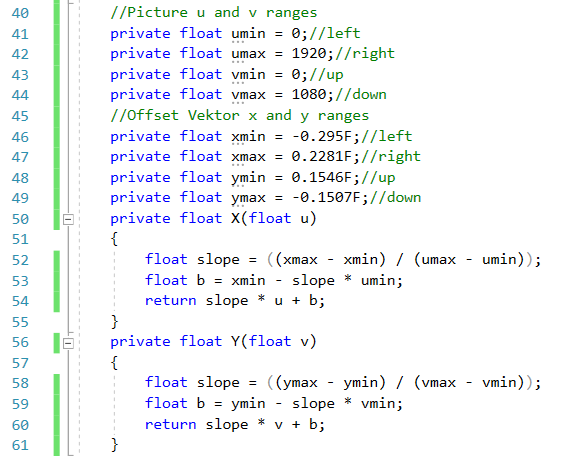
\includegraphics[width=0.5\textwidth]{images/code_uv_to_xy_scale.PNG}
	\caption[]{Funktionen X und Y}
	\label{code:uvtoxy}
\end{figure}

Die Funktionen werden genutzt um die u,v Koordinate eines DetectedObject in einen Offset-Vektor umzuwandeln. Der Offset wird mit der cameraToWorld Matrix multipliziert um den Punkt p im 3D Raum zu erhalten, der sich an der korrekten Stelle auf der Clippling Plane befindet. Siehe Abbildung \ref{code:castmethod}.

\begin{figure}[H]
	\centering
	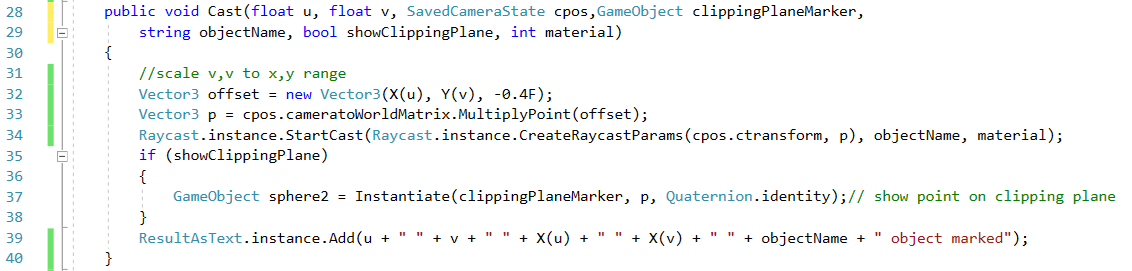
\includegraphics[width=1.1\textwidth]{images/code_cast_method.PNG}
	\caption[]{Cast Methode}
	\label{code:castmethod}
\end{figure}
\subsection{Raycast}

Als Nächstes wird ein Raycast durch den Ursprung der Kamera und den Punkt p gesendet. Dort wo der Raycast auf das Spatial Mapping Mesh trifft, ist das DetectedObject in dem 3D Raum zu finden. 

Das Spatial Mapping Mesh wird von dem MLSpatialMapper erzeugt und bildet die Reale Welt ab. Um ein Raycast auf das Mesh auszuführen, wird MLRaycast eingesetzt. Ein MLRaycast brauch zwei Parameter:
\begin{itemize}
	\item Ein QueryParams Objekt, das Ursprung und Richtung für den Raycast beinhaltet.
	\item Eine Methode die aufgerufen wird, wenn der Raycast fertig ist. 
\end{itemize}
In den QueryParams wird die Kamera als Ursprung für den Raycast angegeben, während ein Richtungsvektor von der Kamera zu dem Punkt p die Richtung des Raycastes bestimmt. Siehe Abbildung \ref{code:raycastparams}.

\begin{figure}[H]
	\centering
	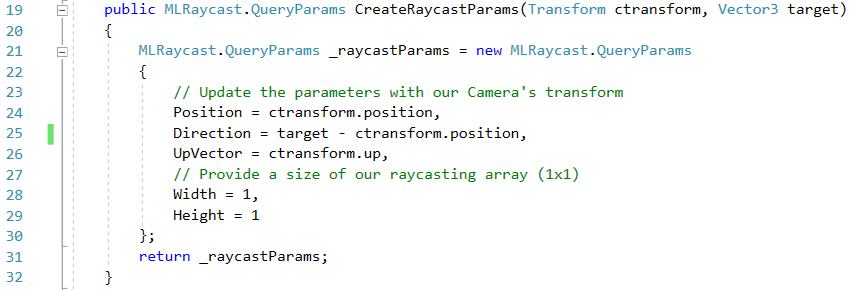
\includegraphics[width=0.7\textwidth]{images/code_raycastparams.PNG}
	\caption[]{Cast Methode}
	\label{code:raycastparams}
\end{figure}

Wenn der Raycast fertig ist, wird die Methode HandleOnRecieveRaycast aufgerufen. Der Parameter point beinhaltet dabei die Koordinate, die getroffen wurde.
Dieser Parameter wird an die Methode CreateMarker von der Klasse LabelCreater weitergegeben.

\subsection{LabelCreater}

CreateMarker erhält den Punkt point der getroffen wurde und die Bezeichnung für das DetectedObject. An der Koordinate von point wird ein Prefab GameObject instanziiert, das als Markierung für das DetectedObject in der 3D Umgebung dient.

Das Prefab besteht aus einer Kugel und einem Schriftzug, der den Namen des DetectedObject anzeigen soll. Dem neu instanziierten GameObject wird die Bezeichnung des DetectedObject als Schriftzug zugewiesen. Siehe Abbildung \ref{image:labels}.

\begin{figure}[H]
	\centering
	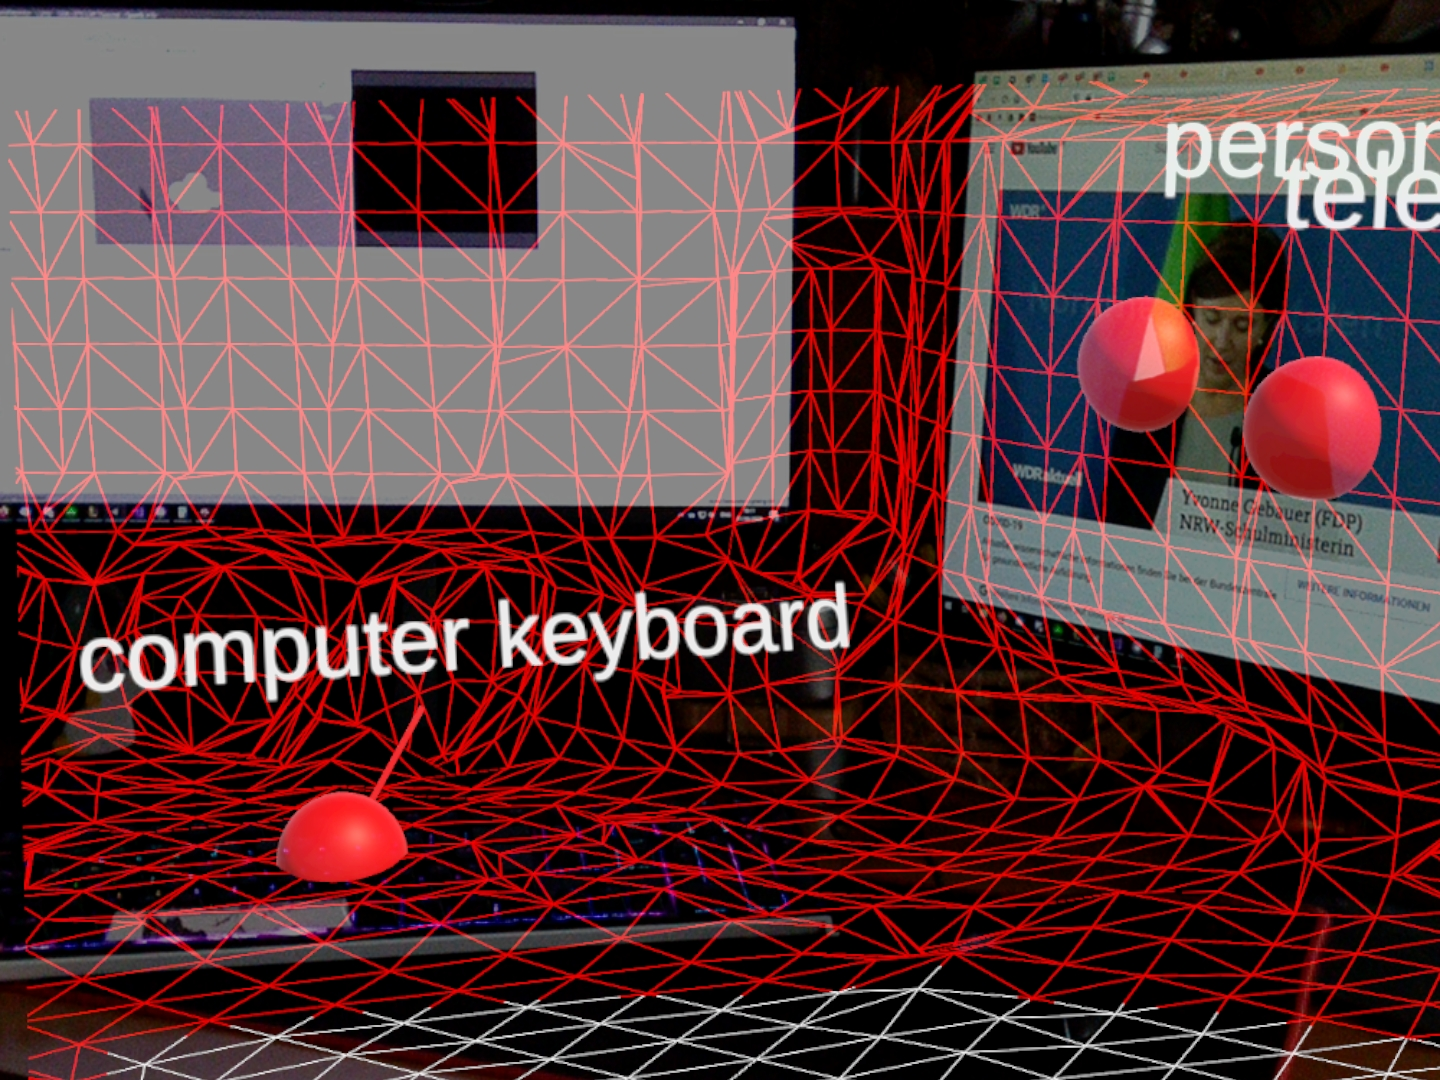
\includegraphics[width=0.7\textwidth]{images/ML_labels.jpg}
	\caption[]{Markierungen in der Welt}
	\label{image:labels}
\end{figure}

\subsection{Azure Custom Vision}

Neben der Bildanalyse mit Azure Object Detection wird auch Azure Custom Vision verwendet.
Die AI wurde über die Webseite trainiert.

Die Anfrage an den Service passiert in der Klasse AzureCustomPrediction. Ähnlich wie bei AzureObjectDetection wird ein Webrequest erstellt mit einem authorization key für den Service und einem Foto als payload.

In der Antwort wird eine Json Datei zurückgeschickt, die die gefundenen Objecte angibt.
Da die Json Datei eine etwas anderes Format hat, wurde eine eigene Handle Json Methode dafür geschrieben.

Für jedes erkannte Objekt wird die Methode Cast von PixelToWorld aufgerufen, um das Objekt in der realen Welt zu lokalisieren und zu markieren.

\subsubsection{Das Trainieren}

Es wurde Probiert das Cusotm Vision Modell auf drei unterschieldiche Objekte zu trainieren.
Dabei wurden vier Iterationen erstellt. 

Iteration 1:

Zunächst wurde probiert Tuben von Acrylfarbe zu erkennen. Die Genauigkeit war davon war nicht so gut. Es wurden in den Fotos Acrylfarben erkannt, wo es keine gab. Sieh Abbildung \ref{image:customVisionPaint}. 

\begin{figure}[H]
	\centering
	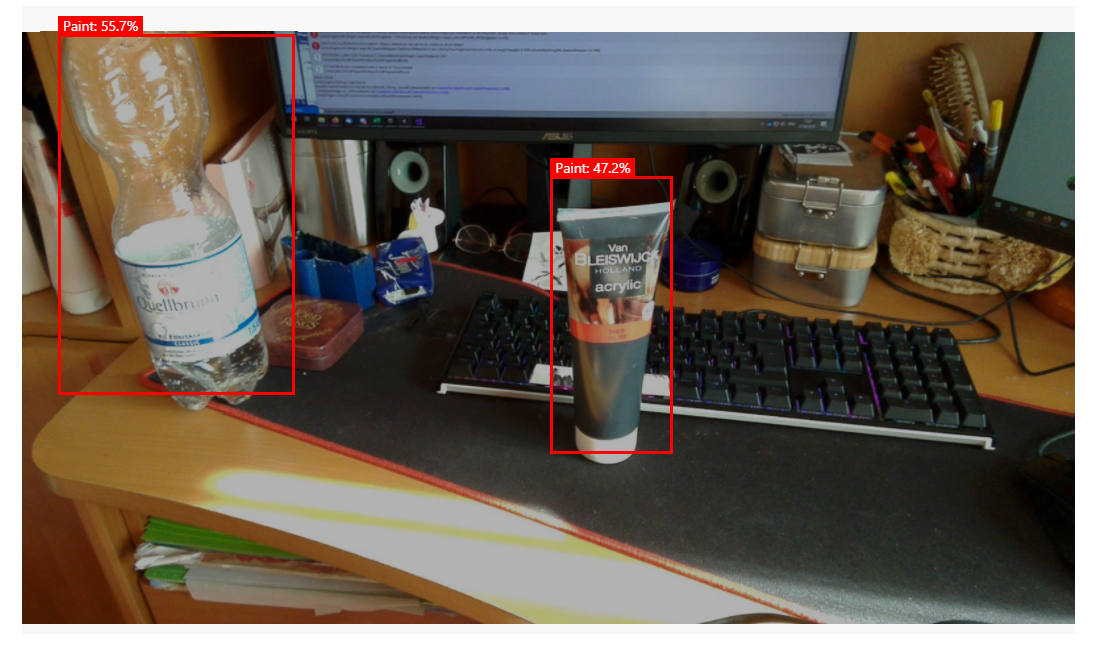
\includegraphics[width=1.0\textwidth]{images/customVisionPaint.PNG}
	\caption[]{Beispielfoto Iteration 1. Die Wasserflasche wurde als Farbe markiert mit 55.7 Prozent statistischer Konfidenz. Die Tatsächliche Farbtube wurde mit einer Konfidenz von 47.5 Prozent erkannt.}
	\label{image:customVisionPaint}
\end{figure}

Iteration 2:

In der zweiten Iteration wurde probiert das Model darauf zu trainieren, eine Blaue Dose von Nivea Hautcreme to erkennen. Die Form und Farbe von der Dose ist sehr simpel, daher wurde davon ausgegangen, das sie leicher zu erkennen ist. Auch dort dar die Genauigkeit zunächt bei nur 80 Prozent. Es wurden in vielen Fotos fälschlicherweise Nivea Dosen erkannt.

Iteration 3:

In der Iteration drei wurde versucht Iteration 2 zu verbessern. Es wurden ausgewählte Training Fotos entfernt, die die Dose von einem Seitlichen Winkel zeigten, mit der mit der Erwartung das die Detektion der Dose aus dem Blickwinkel von Oben damit konsistenter wird. Zusätzlich wurden mehr Fotos von der Dose auf verschieden farbigen und gemusterten Untergrund hinzugefügt. 

Die Genauigkeit der Prediction sank auf 75 Prozent.

Iteration 4:

In Iteration 4 wurden zwei Fotos von der Nivea Dose entfernt, das die Genauigkeit auf 100 Prozent steigen ließ. In der Umsetzung mit der Magic Leap Anwendung werden trotzdem häufig Objekte fälschlicherweise als Nivea Dose markiert.

Neben der Dose wurde diese Iteration darauf trainiert eine bestimmte Holz Haarbürste zu erkennen. Aufgrund von dem komplexeren, und markanten Aussehen der Bürste ist davon ausgegangen, das die Bürste besser von anderen Objekte zu unterschieden ist. 
Die Bürste wurde nur mit den Borsten nach oben Photographiert.

Die Genauigkeit für die Bürste lag bei 100 Prozent. 
In der Umsetzung mit der Magic Leap Anwendung wird die Bürste häufig nicht erkannt, obwohl sie im Bild ist und mit den Borsten nach oben liegt. Es werden jedoch keine Objekte als Haarbürste erkannt die keine sind.

\subsection{Entwicklung von PixelToWorld}
%todo schrieben was ich ausprobiert habe in pixel to world

Zuerst ausprobiert 

virtuell foto abschneiden nur den bereich verwenden, der auch auf dem display zu sehen ist. besseres feedback, das objekte dort entstanden sind und man weiß das dort das mesh schon ist.

dafür ausprobiert, welche pixel des fotos am rand des displays liegen. dafür das zuletzt aufgenommene foto in der Anwendung in einem UI element anzeigen. ein tranzparentes gitternetzt darüber gelegt, wo man ablesen kann, welcher pixel sich wo auf dem foto befindet. Darüber durch Fotos machen und ablesen welche real world features sich bei welcher pixel position befinden. Herausstellen, welcher Fotoausschnitt mit dem Display übereinstimmt. 
%bilder zeigen wie es dann aussieht
%make methods, classes and variables italic

\section{Zusammenfassung}
%sachen die verbessert werden könnten
man kann zusätzlich zum raycast auf das mesh auch noch die tiefenkamera nutzen. spatial mapping hat manchmal das mesh an der stelle noch nicht, oder ist nicht aktualisiert. besonders probleme mit wasserflaschen die nicht erkannt werden. HInzuzihenen von tiefen datan kann das lokalisieren von objekten im 3D raum noch verbessern.
	
	\newpage
	\printbibliography
\end{document}